\newpage
\section{Oppbygging av programmet}
\thispagestyle{fancy}

\subsection{Programmeringsmetode}
For å sette i samen alle funksjonsblokkene vi hadde skreve i \gls{ST}, så valde vi å bruke \GLS{Codesys} Continuous Function Chart (\gls{CFC}).
\gls{CFC} er ein grafisk programmeringsmetode som bruker symbol og koplingar for å gjere programmet  meir visuelt.

Alle samansetningar av blokker valde vi å gjere i \gls{CFC}. Ved å bruke ein grafisk metode sikra vi oss god lesbarheit og
visuell forståelse av programmet. 

Alle inngangar og utgangar er leselege og enkle og forstå. \gls{CFC} i lag med god dokumentasjon vil kunne gi personar utan programmeringsbakgrunn
god forståelse av korleis programmet er bygd opp, utan å måtte lese kodelinjer.
\gls{CFC} gir eit godt grunnlag for feilsøking og analyse, dette bygger derfor vidare på filosofien med eit enkelt og fleksibelt program.

Dersom antall koplingar og linjer gjorde programmet vanskeleg å lese var det også
mogleg å opprette ``source'' og ``links'' som oppretta ein trådlaus forbindelsane gjennom ein unik ID.

\begin{figure}[htbp]
    \centering
    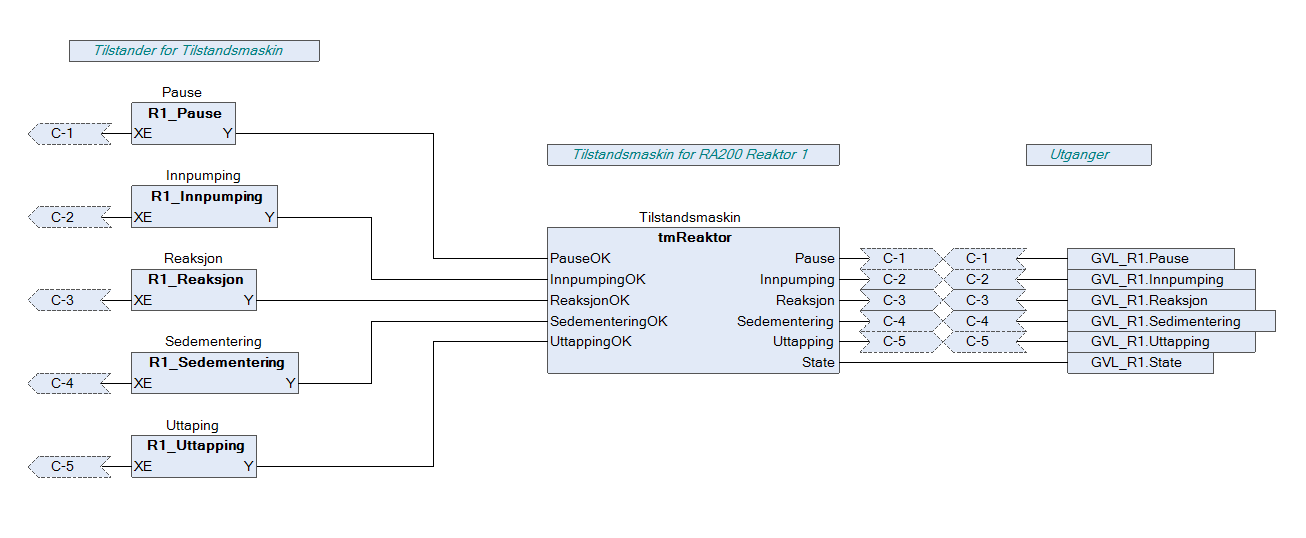
\includegraphics[width=1\textwidth]{Bilder/ReaktorPRG.png}
    \caption{Eksempel \gls{CFC} - Styring reaktor 1}\label{fig:CFCReaktor}
\end{figure}

\newpage

\subsection{Hovuddel}

Programmet er delt opp i tre hovuddelar, ei tilstandsmaskin for kvar reaktor og ein del for samling av felles reaktorfunksjonar.
Alle delane har eit kall i MainTask og blir utført ved kvar \gls{PLS} syklus. Tilstandsmaskina har det overordna ansvaret og passar på kva 
funksjonsblokk med tilstandslogikk som køyrer.

Felles funksjonar er ei samling av funksjonsblokker og utrekningar som er felles for reaktorane, og er uavhengig av tilstandsmaskina til kvar enkelt reaktor.
Driftsovervaking er ein sentral del av felles funksjonar, der gangtid og mengda av prosessert vatn er døme på funksjonar og utrekningar som vert utførte.

I nokre tilfelle, som ved rullering av sivbed, var vi avhengig av at både tilstandsmaskin for reaktor ein og reaktor to hadde den same informasjonen.
Dette løyste vi ved å lage ei funksjonsblokk ``fbSivbedRotation'' i felles funksjonar, som hentar inn og behandlar antall slamuttak for å så rotere sivbed når ei gitt grense er nådd.
Denne informasjonen blir deretter sendt til kvar tilstandsmaskin, som sørger for at begge reaktorane har same aktive sivbedet.

\begin{figure}[htbp]
    \centering
    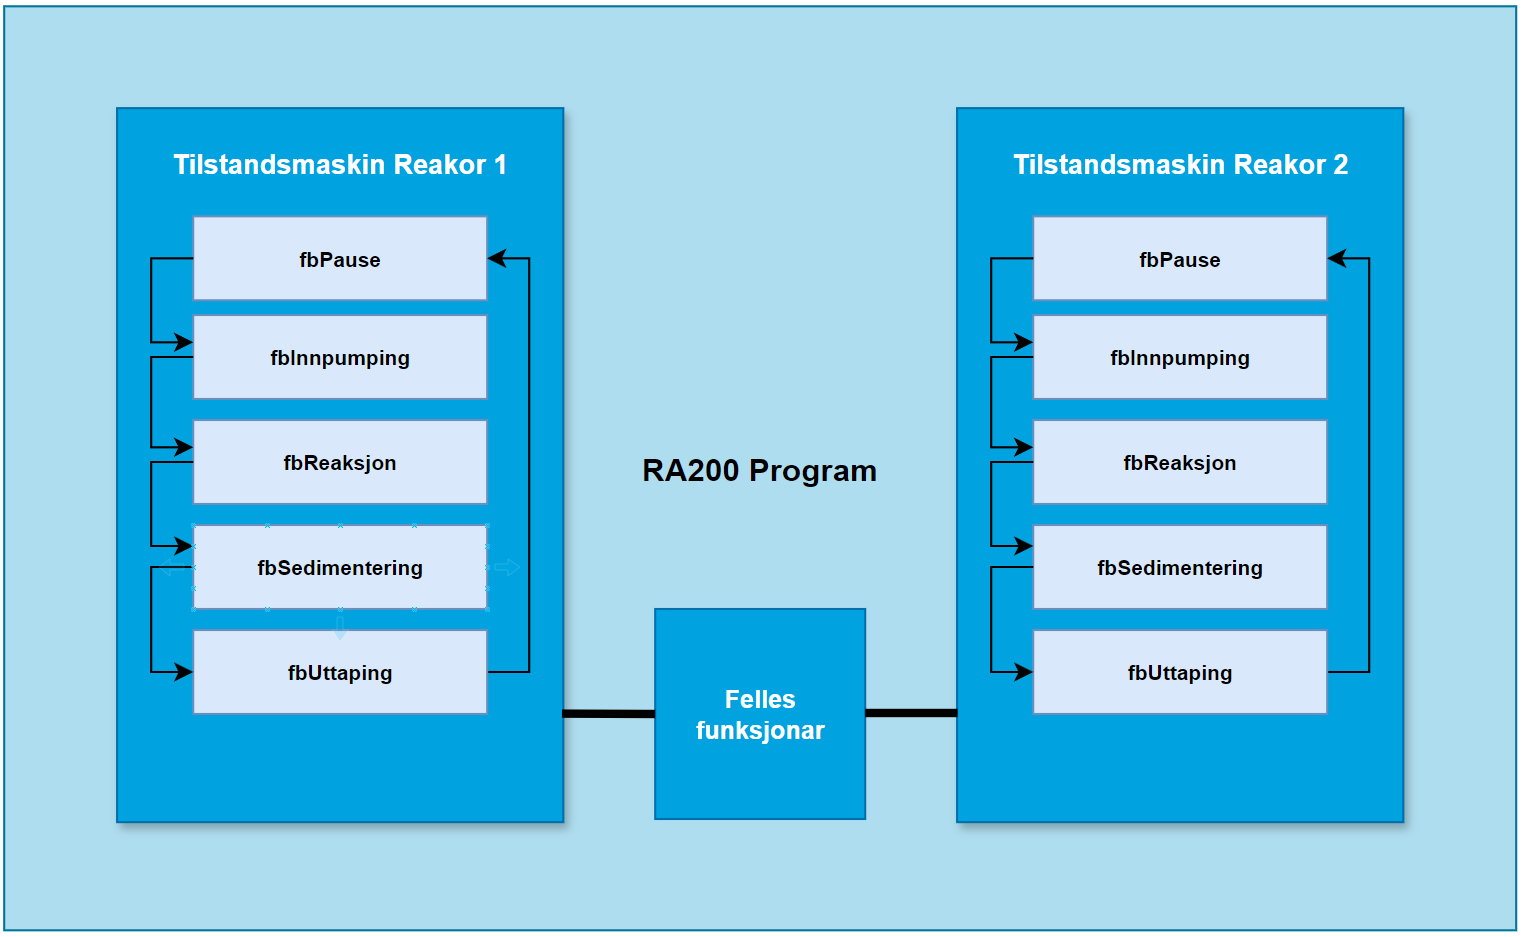
\includegraphics[width=1\textwidth]{Figurar/Oppbygging_Program.png}
    \caption{Illustrasjon oppbygging av programmet}\label{fig:OppbyggingProgram}
\end{figure}

\newpage

\subsection{Styring tilstandslogikk}

Som tidlegare nemnt er det tilstandslogikken som samarbeider opp mot \gls{IEC} blokkene. Dette samarbeidet valde vi også å gjere i eit
\gls{CFC} vindu som gjorde kall og koplingar meir visuelt. \gls{CFC} vinduet fikk namn etter kva sekvens i \gls{SBR}-prosessen
den hadde ansvar for å styre. 

Oppbygginga av desse sekvensstyringane er gjort med inngangsblokker (\gls{MA} og \gls{MB}) øvst og utgangsblokker (\gls{SBE} og \gls{SBV}) i botn av vinduet.
I mellom desse kjem sjølve tilstandslogikkblokka som inneheld styringslogikken.

\begin{figure}[htbp]
    \centering
    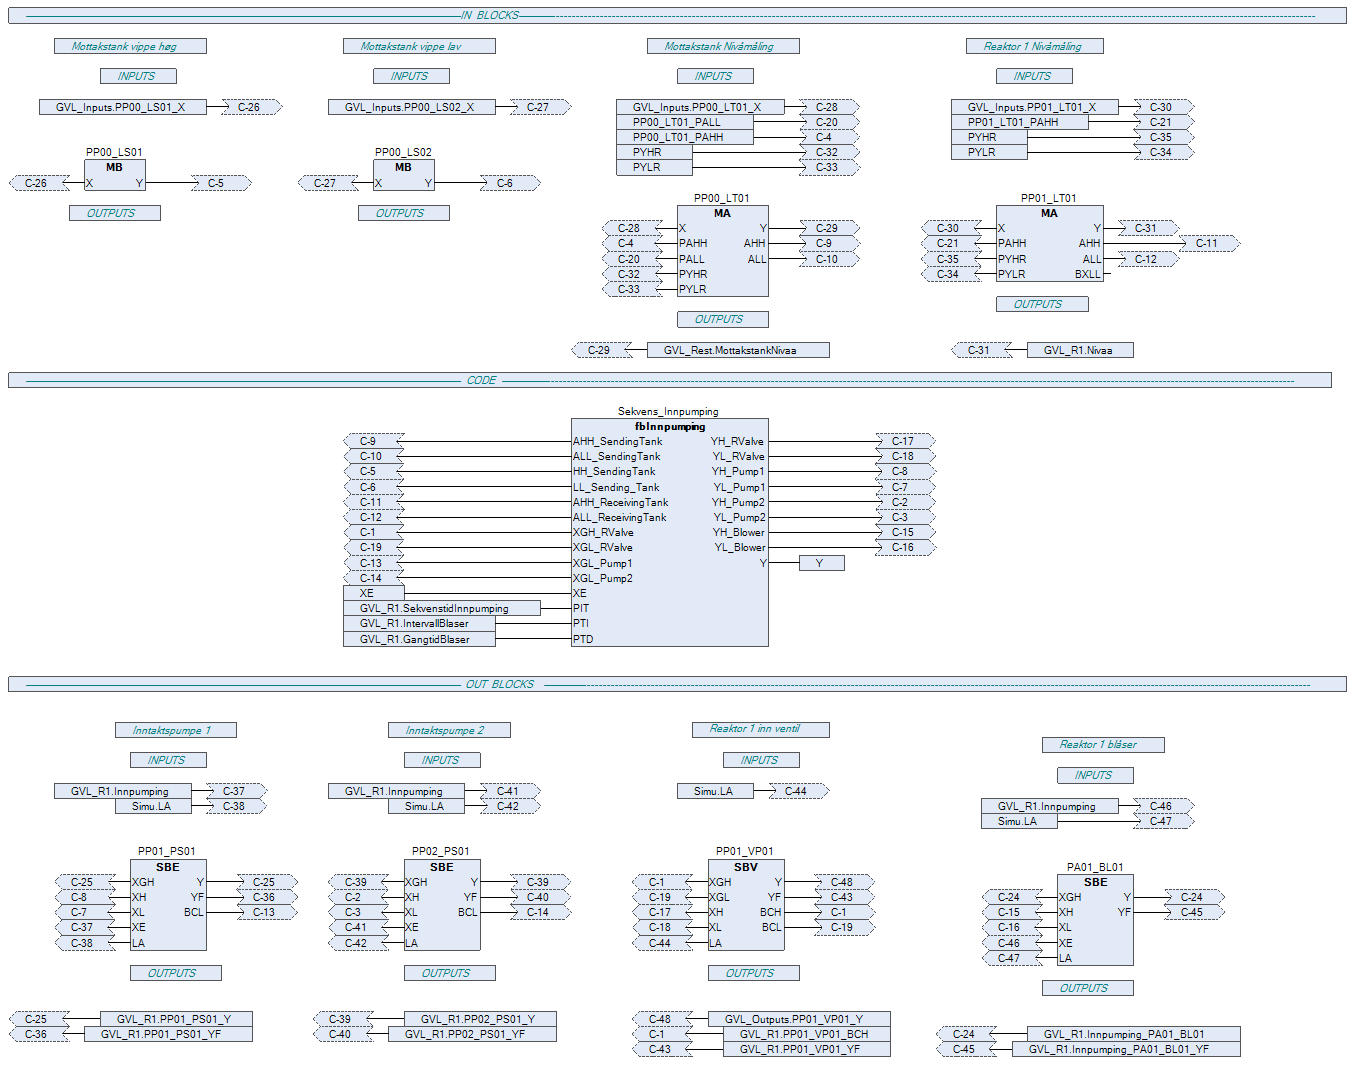
\includegraphics[width=1\textwidth]{Bilder/Heile_innpump.png}
    \caption{Eksempel \gls{CFC} - styring innpumping}\label{fig:CFCInnpumping}
\end{figure}

I denne figuren er ekstra inngangar, parameterinngangar og ekstra utgangar fjerna for å betre kunne visualisere koplingane og samarbeidet mellom
\gls{IEC} blokkene og funksjonsblokka for tilstandslogikken.

\newpage

